\section{Modern Models}\label{sec:models}
This section contains an overview of selected modern models used extensively in facial recognition tasks.

\subsection{InceptionNet}\label{subsec:inceptionnet}
InceptionNets are a class of models in which there are multiple kernel sizes operating at the same level.
This is desirable because the right kernel size is dependent on how globally the information is distributed.
A large kernel is preferred when the information is distributed globally and, vice versa.

\begin{figure}[H]
    \centering
    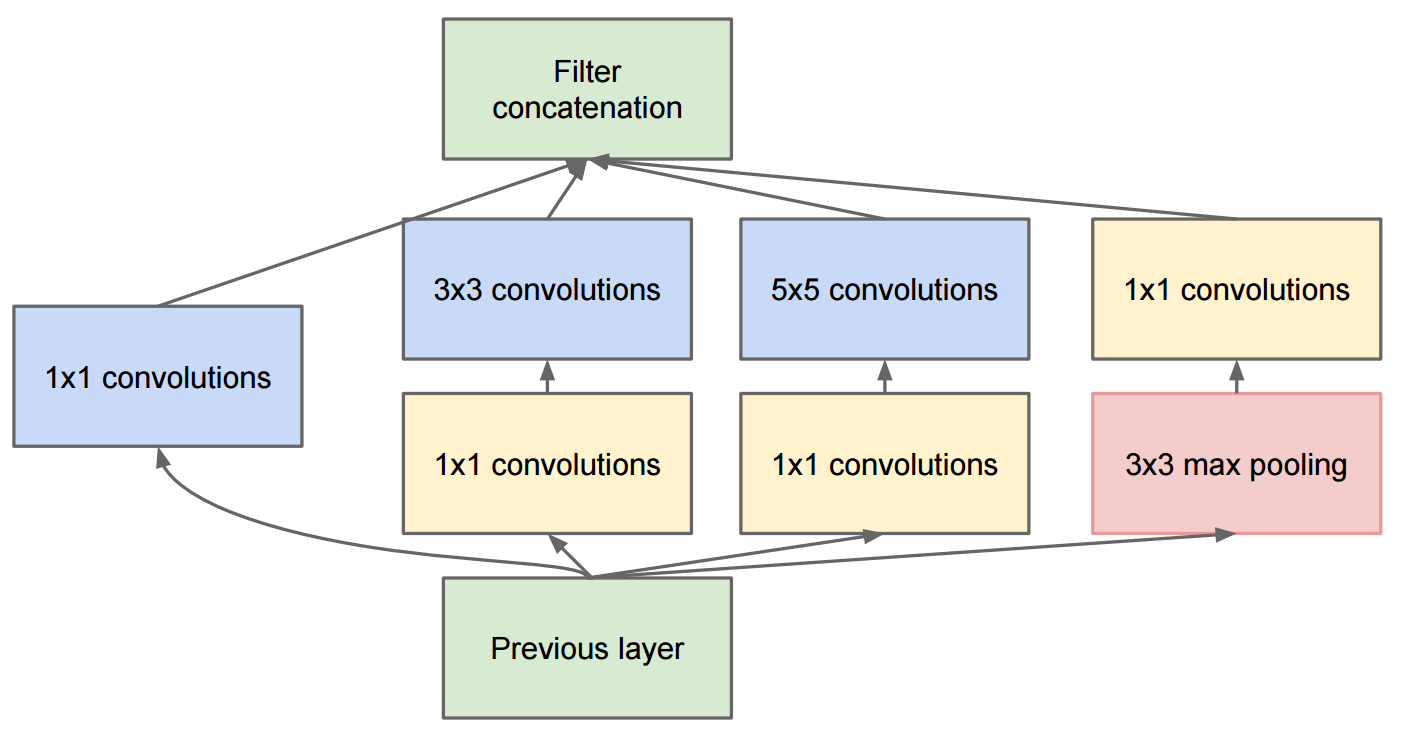
\includegraphics[width=0.9\columnwidth]{images/face-recognition/inceptionnet.png}
    \caption{InceptionNet block~\cite{GoingDeeper}}
    \label{fig:InceptionNet}
\end{figure}

The inception of the inception block (figure~~\ref{fig:InceptionNet}) took place in 2014 in the paper~\cite{GoingDeeper}
published by Google Inc.
Models using inception blocks kept on improving and at the time of writing, there is the fourth version in use.

\subsection{ResNet}\label{subsec:resnet}
A residual neural network (ResNet)~\cite{ResNet} is an ANN which allows for the training of
very deep neural networks containing tens of layers.
Training of ANNs this deep had been practically impossible before the invention of ResNet due to the problem of
\textit{vanishing gradient} and \textit{degradation problem}.
The first problem is exposed as a lack of convergence and the second one as a high training error.

Both of these problems have been avoided by implementation of \textit{skip connections} which are illustrated in the
figure~\ref{fig:ResNet}.

\begin{figure}[H]
    \centering
    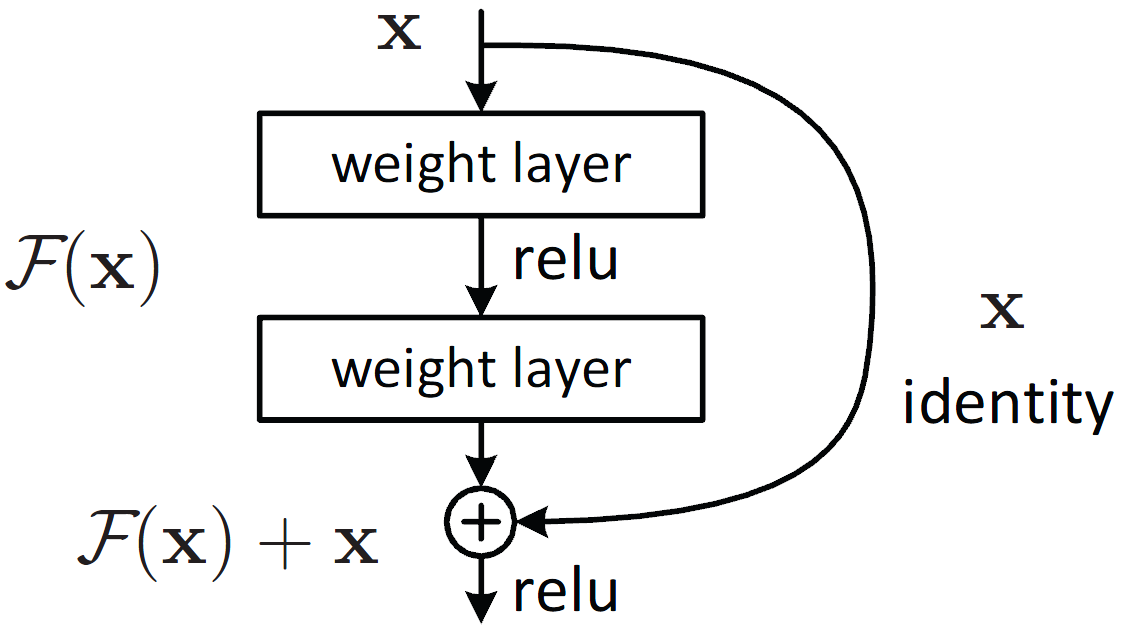
\includegraphics[width=0.9\columnwidth]{images/face-recognition/resnet.png}
    \caption{Residual learning~\cite{ResNet}}
    \label{fig:ResNet}
\end{figure}

The skip connections are implemented as elementwise addition and they let the in-between layers fit a residual mapping.

ResNets are widely used in the field of facial recognition as well as in the field of computer vision as a whole.

In the experimental part, I use 18-layer version called ResNet-18 (see section~\ref{ch:implementation}).

\subsubsection{Architecture of ResNet-18}\label{subsubsec:resnet18}
In the architecture, there are 17 convolutional layers and 1 dense layer.
As is usual, the dense layer is placed at the output.
Each of these layers is followed by batch normalization.
The dimensionality of the first layer's feature map is reduced by max pooling.
ReLu is used extensively within the whole architecture.

\subsection{DenseNet}\label{subsec:densenet}
DenseNet~\cite{DenseNet} is a type of CNN~\ref{ch:cnn} which was introduced in 2017.
The difference from regular CNNs is that every layer is connected to all the subsequent layers.
Traditional CNN with \textit{L} layers has exactly \textit{L} connections.
On the other hand DenseNet with the same amount of layers contains $\frac{L\left( L+1 \right)}{2}$ connections.
The block of layers is illustrated in the figure~\ref{fig:DenseNet}.

\begin{figure}[H]
    \centering
    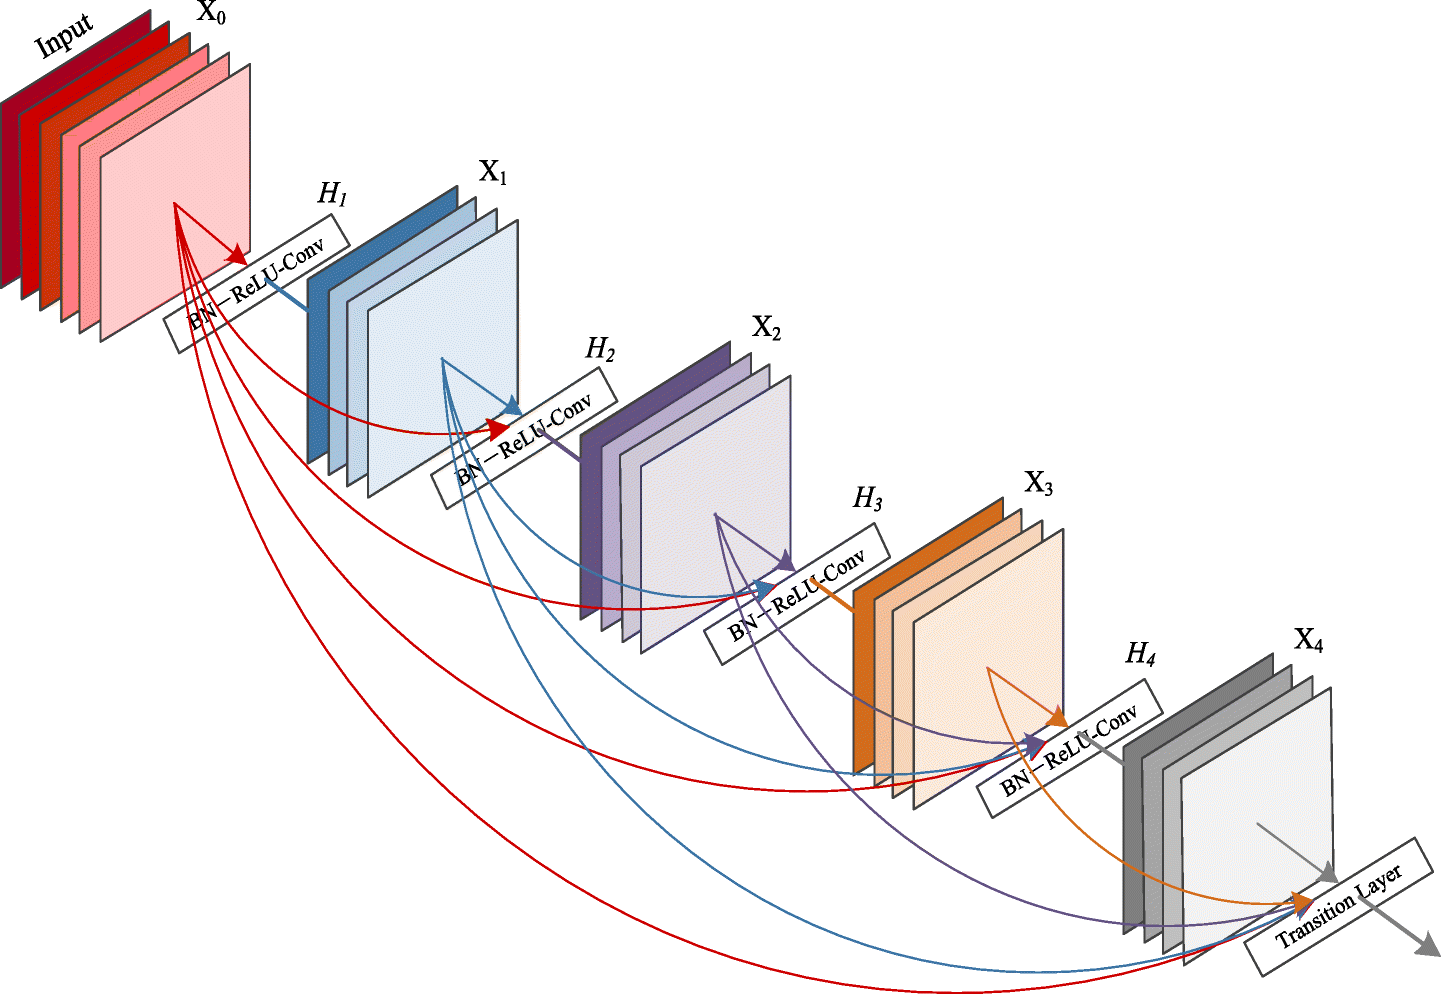
\includegraphics[width=0.9\columnwidth]{images/face-recognition/densenet.png}
    \caption{A 5-layer dense block~\cite{DenseNet}}
    \label{fig:DenseNet}
\end{figure}

DenseNets implement the connections with preceding layers differently than ResNets.
While ResNets use elementwise addition, DenseNets concatenate the feature maps.
The big size of the feature map is not an issue because it is fed as an input into a convolutional layer,
and consequently, the training does not require training more parameters.

DenseNets have several compelling advantages~\cite{DenseNet}.
They alleviate the vanishing-gradient problem, strengthen feature propagation, encourage feature reuse, and
substantially reduce the number of parameters.